\documentclass[12pt]{article}
 
\usepackage[margin=.75in]{geometry} 
\usepackage{amsmath,amsthm,amssymb}
\usepackage{bm}
\usepackage{enumitem}
\usepackage{color}
\usepackage{graphicx}
\usepackage{verbatim}
\setenumerate{listparindent=\parindent}
\definecolor{gray}{gray}{0.6}

\setenumerate{listparindent=\parindent}
 
\newcommand{\N}{\mathbb{N}}
\newcommand{\Z}{\mathbb{Z}}
\newcommand{\E}{\mathbb{E}}
\DeclareMathOperator*{\Cov}{Cov}
\DeclareMathOperator*{\Col}{Col}
 

\newcommand*{\thead}[1]{\multicolumn{1}{|c|}{\bfseries #1}}

\usepackage{listings}
\lstset{
language=R,
basicstyle=\scriptsize\ttfamily,
commentstyle=\ttfamily\color{gray},
%numbers=left,
numberstyle=\ttfamily\color{gray}\footnotesize,
stepnumber=1,
numbersep=5pt,
backgroundcolor=\color{white},
showspaces=false,
showstringspaces=false,
showtabs=false,
frame=single,
tabsize=2,
captionpos=b,
breaklines=true,
breakatwhitespace=false,
%title=\lstname,
escapeinside={},
keywordstyle={},
morekeywords={}
} 

%\usepackage{fancyhdr} % Required for custom headers 
%%\usepackage{lastpage} % Required to determine the last page for the footer
%
%\pagestyle{fancy}
%\lhead{Stat 151A (HW4)}
%\chead{Michael Knopf (24457981)}
%\rhead{April $13^\text{th}$, 2015}
%\lfoot{}
%\cfoot{}
%\rfoot{}
%%\rfoot{Page\ \thepage\ of\ \pageref{LastPage}}
%\renewcommand\headrulewidth{0.4pt}
%%\renewcommand\footrulewidth{0.4pt}


\begin{document}
\title{Modeling Median Home Values in Boston \\ Stat 151A}
\author{Michael Knopf}
 
\maketitle

\section{Introduction}

In attempt to model the median value of owner-occupied homes in the Boston area, we will assume this quantity varies linearly with some or all of the variables listed in the following section, up to the presence of random, uncorrelated errors that normally distributed with mean zero and constant variance.

In our initial analysis, we will identify and attempt to remedy the challenges presented by the data.  Mainly, these challenges consist of contradictions to these assumptions, but another issue that arises is skew.  Next, we will apply various variable selection methods in order to choose the best model.  The criteria we will use combine measures of accuracy and overfitting in order to produce the model that will best predict median home value for new obervations.  Next, we will attempt to eliminate outlier observations from the model.  Finally, we will perform diagnostics on the chosen model, again testing for contradictions of our initial assumptions and evaluating its overall performance.

Once the model has been produced and tested, we will attempt to interpret its results.  Note that the model we seek throughout the majority of this process is the one that predicts best, though this will not necessarily be the one that explains best.  The first model we will produce is meant to answer the simple question, ``Given a new region with values $x_i$ in each of some $p$ categories, what is our best prediction for the median value of owner-occupied homes in that region?"

Other questions we have are about the factors that \emph{cause} home values to be high in one area, but low in another.  Which independent variables have the highest influence on home values?  If city council is trying to raise the median home value in their town, what should be their target areas for improvement?  Should they hire more teachers, or more police officers?  Should they raise or lower taxes?  Should they create incentives to build larger homes, or enact laws to improve the air quality?  There is no doubt that most of these actions would have a positive effect on home values, but which produce the greatest outcome in proportion to their cost?

The model that does best at prediction will actually prove to be relatively ineffective in answering these sorts of questions.  To find answers to these sorts of questions, we will need to investigate smaller models.  In order to keep the length of this report to a minimum, I will mainly discuss the steps I took to produce the first model, the one tailored for prediction value.  However, I will also share one smaller model I have produced, in order to show how it is more applicable to these sorts of inquiries.

%This is a perfectly practical question, but it would likely be a question asked by someone who literally has some area in mind that he or she needs to know the median home value for.
\section{Data}

We will be working with the BostonHousing2 dataset in R.  The data consists of $506$ observations on $19$ variables.  \emph{medv} is the the target variable.  A dictionary of the variables is given below.
\begin{center}
\renewcommand{\arraystretch}{1.2}
\begin{tabular}{|l|l|}
\hline
\thead{Variable} & \thead{Description} \\
\hline 
town & name of town \\ 
\hline 
tract & census tract \\ 
\hline 
lon & longitude of census tract \\ 
\hline 
lat & latitude of census tract \\ 
\hline 
medv & median value of owner-occupied homes in USD 1000's \\ 
\hline 
cmedv & corrected median value of owner-occupied homes in USD 1000's \\ 
\hline 
crim & per capita crime rate by town \\ 
\hline 
zn & proportion of residential land zoned for lots over 25,000 sq.ft \\ 
\hline 
indus & proportion of non-retail business acres per town \\ 
\hline 
chas & Charles River dummy variable (= 1 if tract bounds river; 0 otherwise) \\ 
\hline 
nox & nitric oxides concentration (parts per 10 million) \\ 
\hline 
rm & average number of rooms per dwelling \\ 
\hline 
age & proportion of owner-occupied units built prior to 1940 \\ 
\hline 
dis & weighted distances to five Boston employment centres \\ 
\hline 
rad & index of accessibility to radial highways \\ 
\hline 
tax & full-value property-tax rate per USD 10,000 \\ 
\hline 
ptratio & pupil-teacher ratio by town \\ 
\hline 
b & $1000(B - 0.63)^2$ where B is the proportion of blacks by town \\ 
\hline 
lsat & percentage of lower status of the population \\ 
\hline 
\end{tabular} 
\end{center}

An initial glance at the data reveals that $medv = cmedv$ for all but 8 tracts, thus only one of these variables should be used (although the documentation seems to imply that $cmedv$ is more current, we will use $medv$ because the assignment specifically says to model this variable).  Some of the most highly correlated variable pairs are $(rad,tax)$, $(nox,indus)$, and $(nox,dis)$, which have correlations of $0.910$, $.764$, and $-.769$, respectively.  Beyond these, many high correlations are present.  This will be a constant challenge, as we run the risk of multicollinearity in our model.

\section{Analysis}

\subsection{Preliminary Analysis of the Data}

\begin{figure}[ht!]
\centering
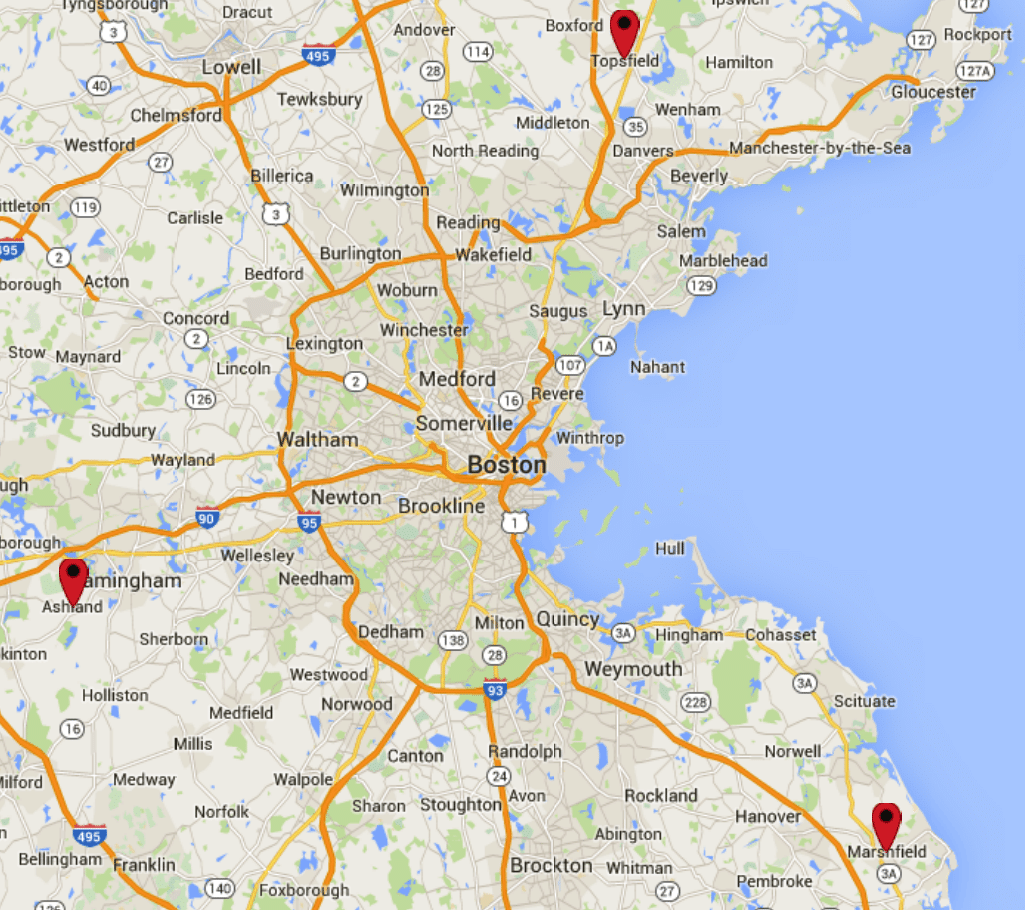
\includegraphics[width=120mm]{map.png}
\caption{The three most extreme regions for which data were collected are plotted here: Topsfield, Marshfield, and Ashland.}
\end{figure}

The dataset includes the variables $lon$ and $lat$, which give the geographic position of each observed tract.  The map in Figure 1 contains markers at the northernmost, westernmost, and easternmost tracts in the dataset (the southernmost point lies directly next to the easternmost point, Marshfield).  The observations are more or less evenly spread throughout a radius around central Boston.  It is intuitive that position \emph{relative to the central city}, rather than absolute vertical and horizontal position, is the better indicator of home value, and further analysis has confirmed this fact.  Therefore, I have substited for these variables with two new ones, defined as
\begin{align*}
londist &= |lat + 71.0589| \\
latdist &= |lon - 42.3601|
\end{align*}
since the heart of the city is located at $(-71.0589,42.3601)$ (I have taken them in absolute value simply because they have proven to perform better this way).

\begin{figure}[ht!]
\centering
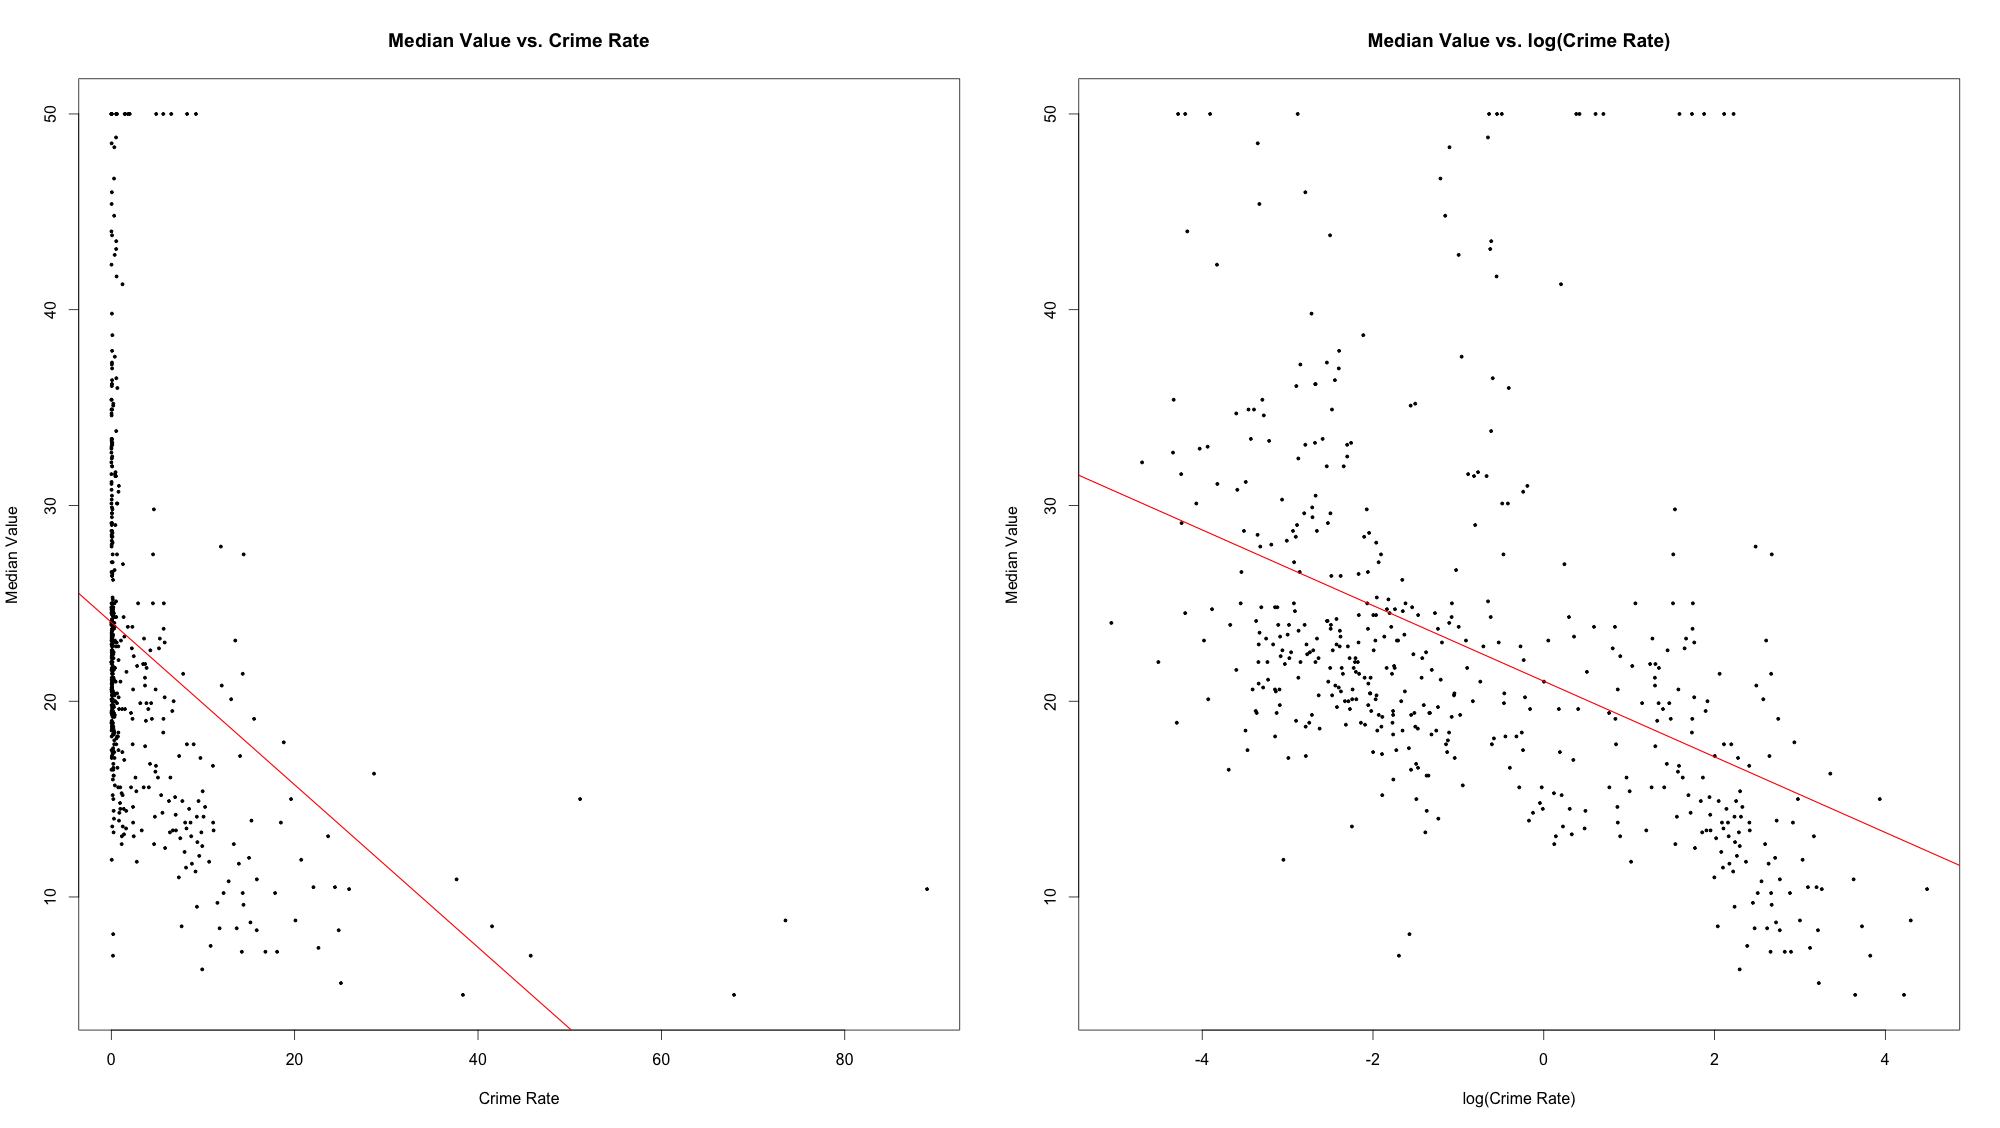
\includegraphics[width=150mm]{crimplot.png}
\caption{The effects of a logarithmic transformation on the left-skewed variable $crim$.}
\end{figure}

Another aspect of the data deserving attention is skewed variables.  Most variables have an acceptable degree of symmetry, though some do show a notable skew.  In particular, the variable $crim$ (crime rate) is heavily skew left.  $65.6\%$ of the values fall below $1\%$, and the frequency thins rapidly as values rise.  I have considered variable transformations to fix this issue; in particular I have tested models that use $\log(crim)$ as a substitue.  Figure 2 shows the effects of this transformation on the relationship between the variable and $medv$.

However, once this transformation has been performed, none of my variable selection methods prefer to keep the variable in the model.  I have decided to leave this data as is.  One justification for this is the argument that crime rates below $1\%$ are effectively indistinguishable from each other.  Areas with crime rates this low are seen as essentially safe; as we move into more dangerous areas, crime increases more than linearly, yet the value of owner-occupied homes \emph{does} decrease proportionately with this non-linear rise.

I have fit $medv$ against each explanatory variable separately.  These plots are given in Figure 3.  Most variables exhibit signs of a linear relationship, though some do not.  Three variables I have looked at intensively are $dis$, $tax$, and $rad$.

\begin{figure}[ht!]
\centering
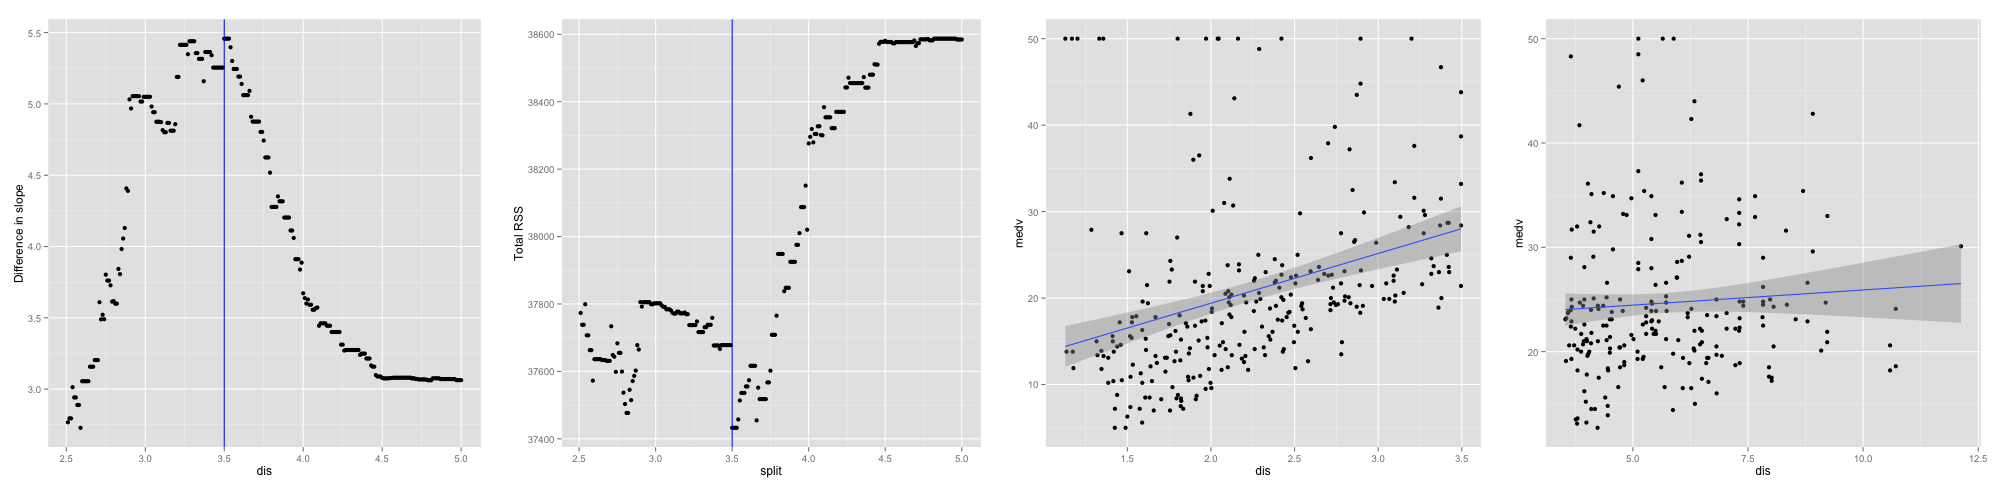
\includegraphics[width=180mm]{displot.png}
\caption{The left two plots show the effects of splitting the data at different values of $dis$.  The right two plots are the corresponding simple linear fits after dividing the data based on whether $dis < 3.5$ (left) or $dis \geq 3.5$ (right).}
\end{figure}

\begin{figure}[ht!]
\centering
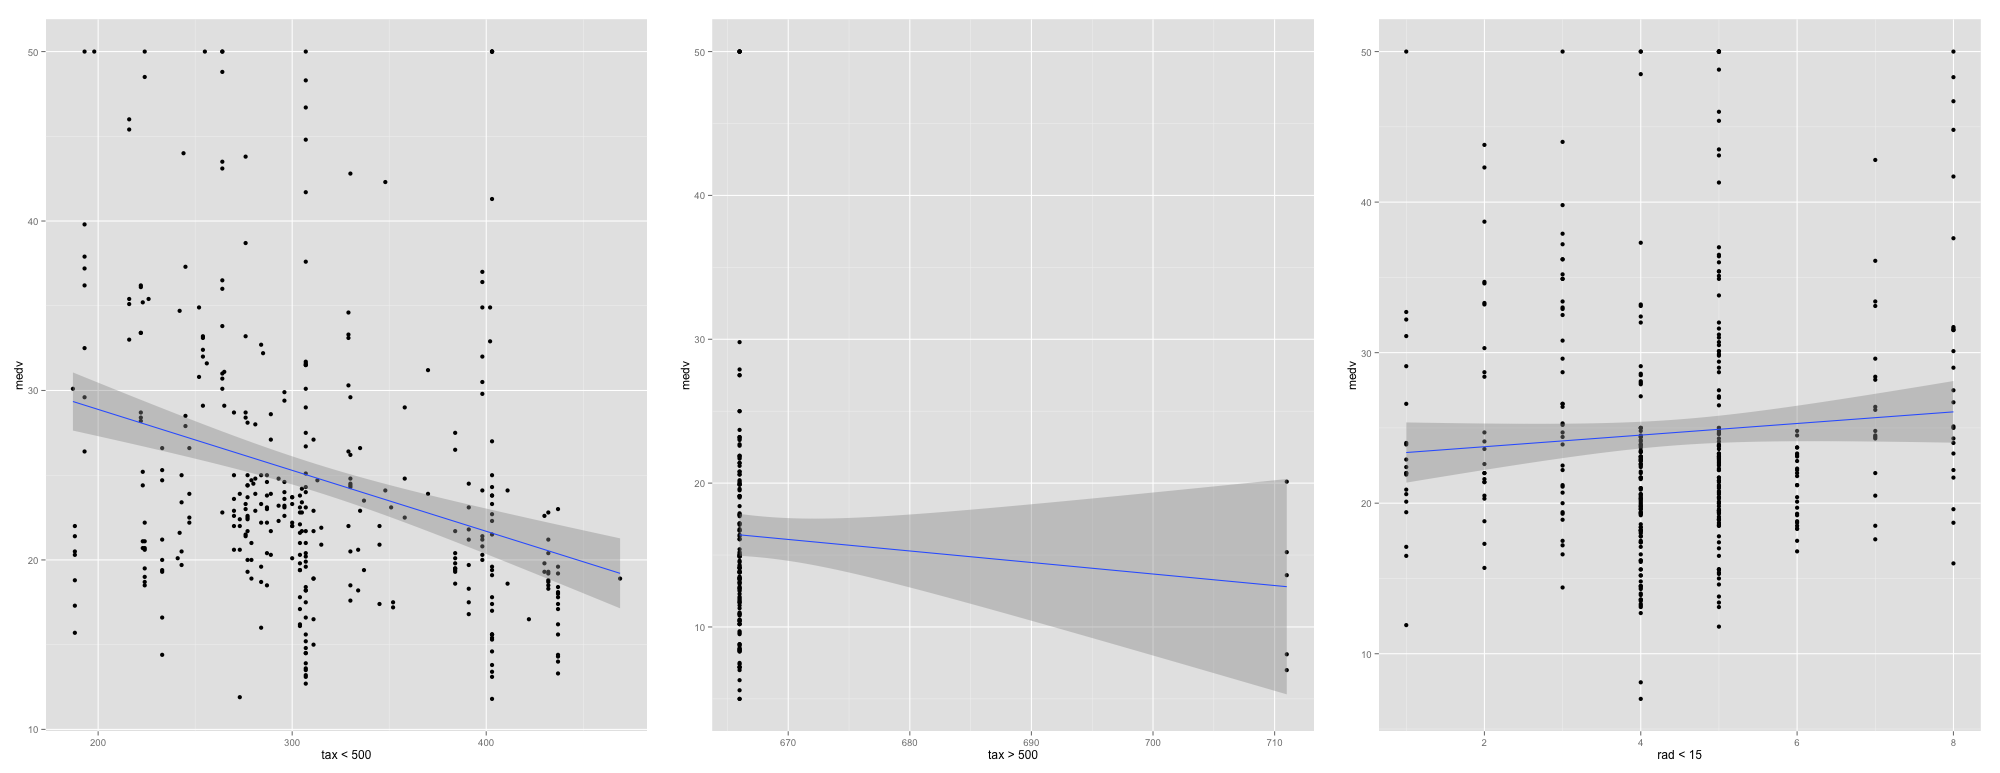
\includegraphics[width=150mm]{taxrad.png}
\caption{Simple linear regression against tax and rad using subsets of the data based on natural splits according to these variables.}
\end{figure}

It appears that $medv$ relates differently to $dis$ depending on whether or not $dis < 3.5$.  For observations with $dis < 3.5$, the coefficient of $dis$ in the simple linear regression model is significantly higher than those for which $dis > 3.5$.  Figure 4 provides plots related to this issue.  The left two plots were useful in identifying 3.5 as the natural value to split the data at.  I tested 250 possible split values ranging between $2.5$ and $5$.  For each of these values, I fit the data separately for observations above and below the split.  The leftmost plot is the resulting difference in slope between the two models.  The next plot is the sum of the squared residuals from both of the models.  3.5 was the value that resulted both in the greatest difference in slope and the lowest total RSS.  The two right plots show the simple linear fits for data above and below this value.  To reflect this issue, I added the interaction term $(dis < 3.5) \cdot dis$ to the model.  Although it was significant in some smaller models, overall it did not seem to be useful, so I have eliminated it from the full model.  I have done a similar analysis for the variables $tax$ and $rad$ (see Figure 5), however the results were similar and I have ultimately left them in the full model as they were.

Finally, I have made plots of the explanatory variables against one another, given in Figure 6.  Unfortunately, some of these plots show significant relationships among the chosen explanatory variables.  This issue is discussed further in Section 4.2.




\subsection{Variable Selection}
The full model of study is
\begin{align*}
\text{MEDV} &= \text{LATDIST + LONDIST + CRIM + ZN + CHAS + NOX + RM} \\
& \text{\ \ + DIS + RAD + TAX + PTRATIO + B + LSTAT.}
\end{align*}
I have run several variable selection procedures in order to select the best submodel.  These procedures were
\begin{enumerate}
\item Backward selection using pValue as criteria.
\item Forward selection using pValue as criteria.
\item Backward selection using Mallow's $C_p$ as criteria.
\item Backward selection using Adjusted $R^2$ as criteria.
\item The step function using AIC as criteria.
\item The step function using BIC as criteria.
\end{enumerate}
The 4th method, using Adjusted $R^2$, produced the model
\begin{align*}
\text{MEDV} &= \text{LATDIST + LONDIST + CRIM + ZN + NOX + RM} \\
& \text{\ \ + DIS + RAD + TAX + PTRATIO + B + LSTAT}
\end{align*}
Every other method produced the model
\begin{align*}
\text{MEDV} &= \text{LONDIST + CRIM + ZN + NOX + RM + DIS} \\
& \text{\ \ + RAD + TAX + PTRATIO + B + LSTAT.}
\end{align*}
which differs only by its exclusion of $latdist$.

\begin{figure}[ht!]
\centering
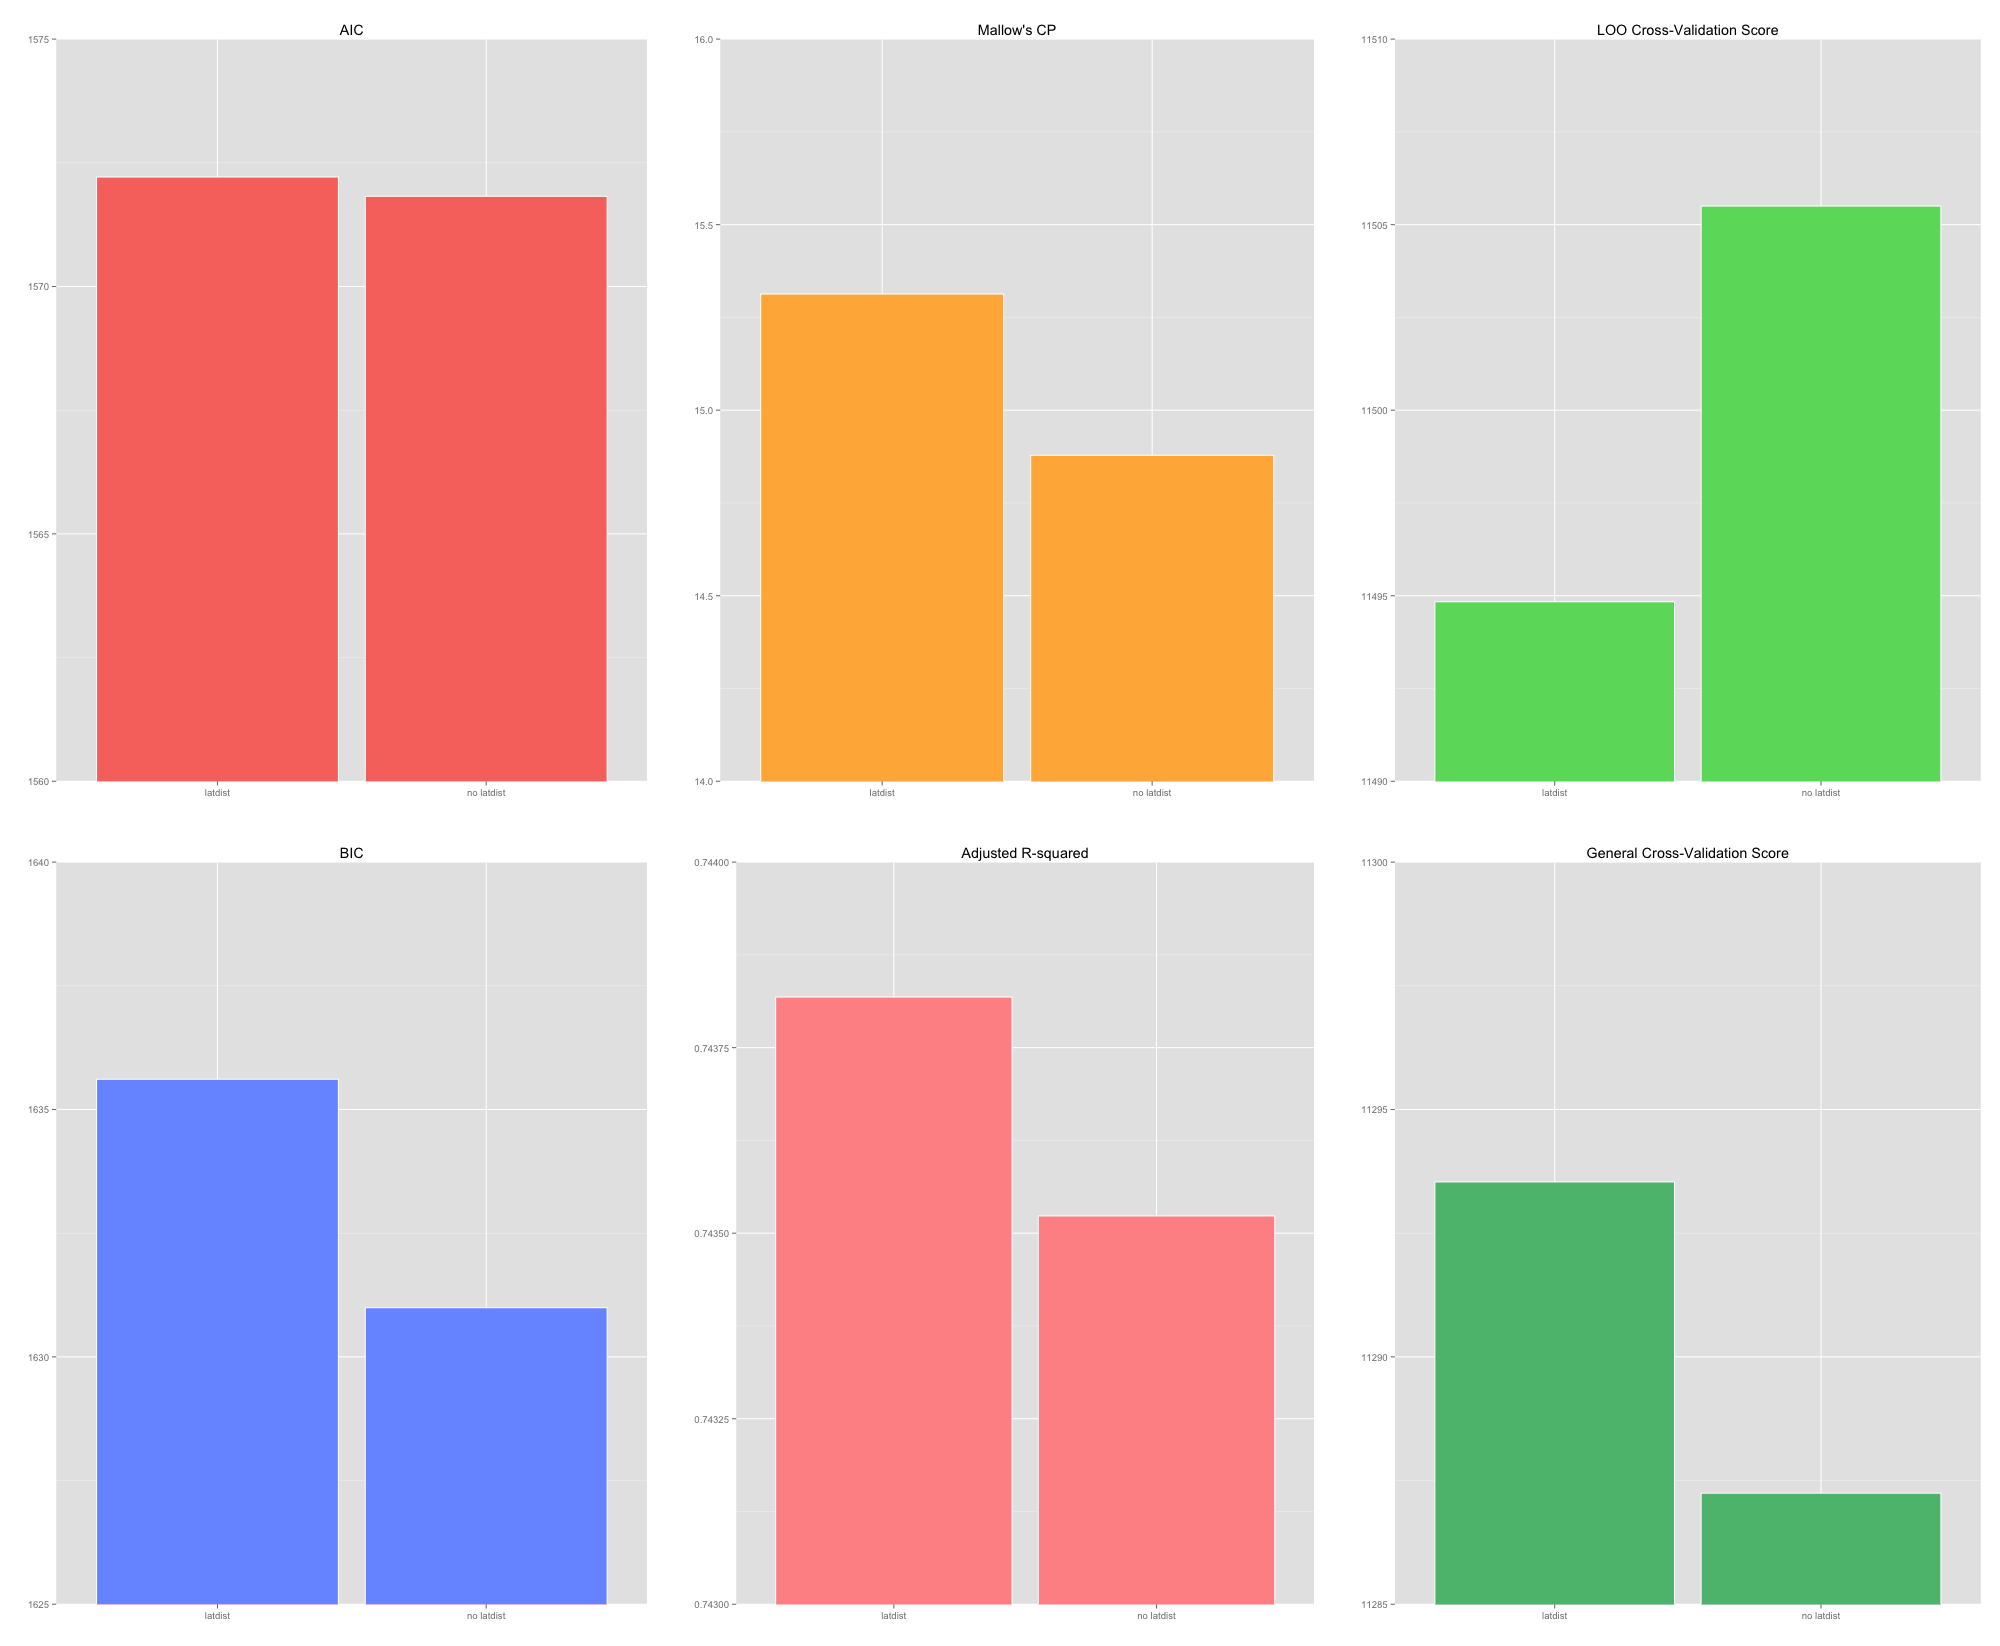
\includegraphics[width=150mm]{barplots.png}
\caption{Model comparison based on selection criteria and leave-one-out cross-validation.  The left model includes $latdist$ while the right model does not.}
\end{figure}

Figure 3 displays the comparison of these two models based on the criteria used for selection, as well as their leave-one-out and general cross-validation scores.  All criteria except for LOO cross-validation prefer the smaller model.  Futhermore, $latdist$ does not show any significant relationship with $medv$ when considered in simple linear regression (see Figure 3).  Overall, it does not appear that the predictive value of the smaller model is significantly less than that of the larger one, especially in light of the risk of overfitting.  I have chosen the smaller model as my final fit.

\subsection{Regression Diagnostics}

I have used the diagnostic plots in Figure 9 to evaluate the assumptions of the linear model.  The plot of the residuals against the fitted values shows hints of nonlinearity, since the scatter has a concave upward shape.  However, the qq-plot of the residuals against the normal quantiles does show that the residuals are approximately normal, though somewhat right skewed.  The plots of the residuals against each explanatory variables (as well as against the fitted values) does support the assumption of constant variance.  Some of these plots appear to have a larger range on one side than the other, but this is due to skewed data rather than nonconstant variance (compare these plots with those in Figure 8 to see that these instances line up with those of uneven distributions of expanatory variables).

I have performed t-tests on each observation to determine whether its standardized predicted residual is significant.  The resulting p-values are plotted in Figure 6, and I have identified and removed those that fall below the critical line of $.05$ (after applying the Bonferroni correction).

\begin{figure}[ht!]
\centering
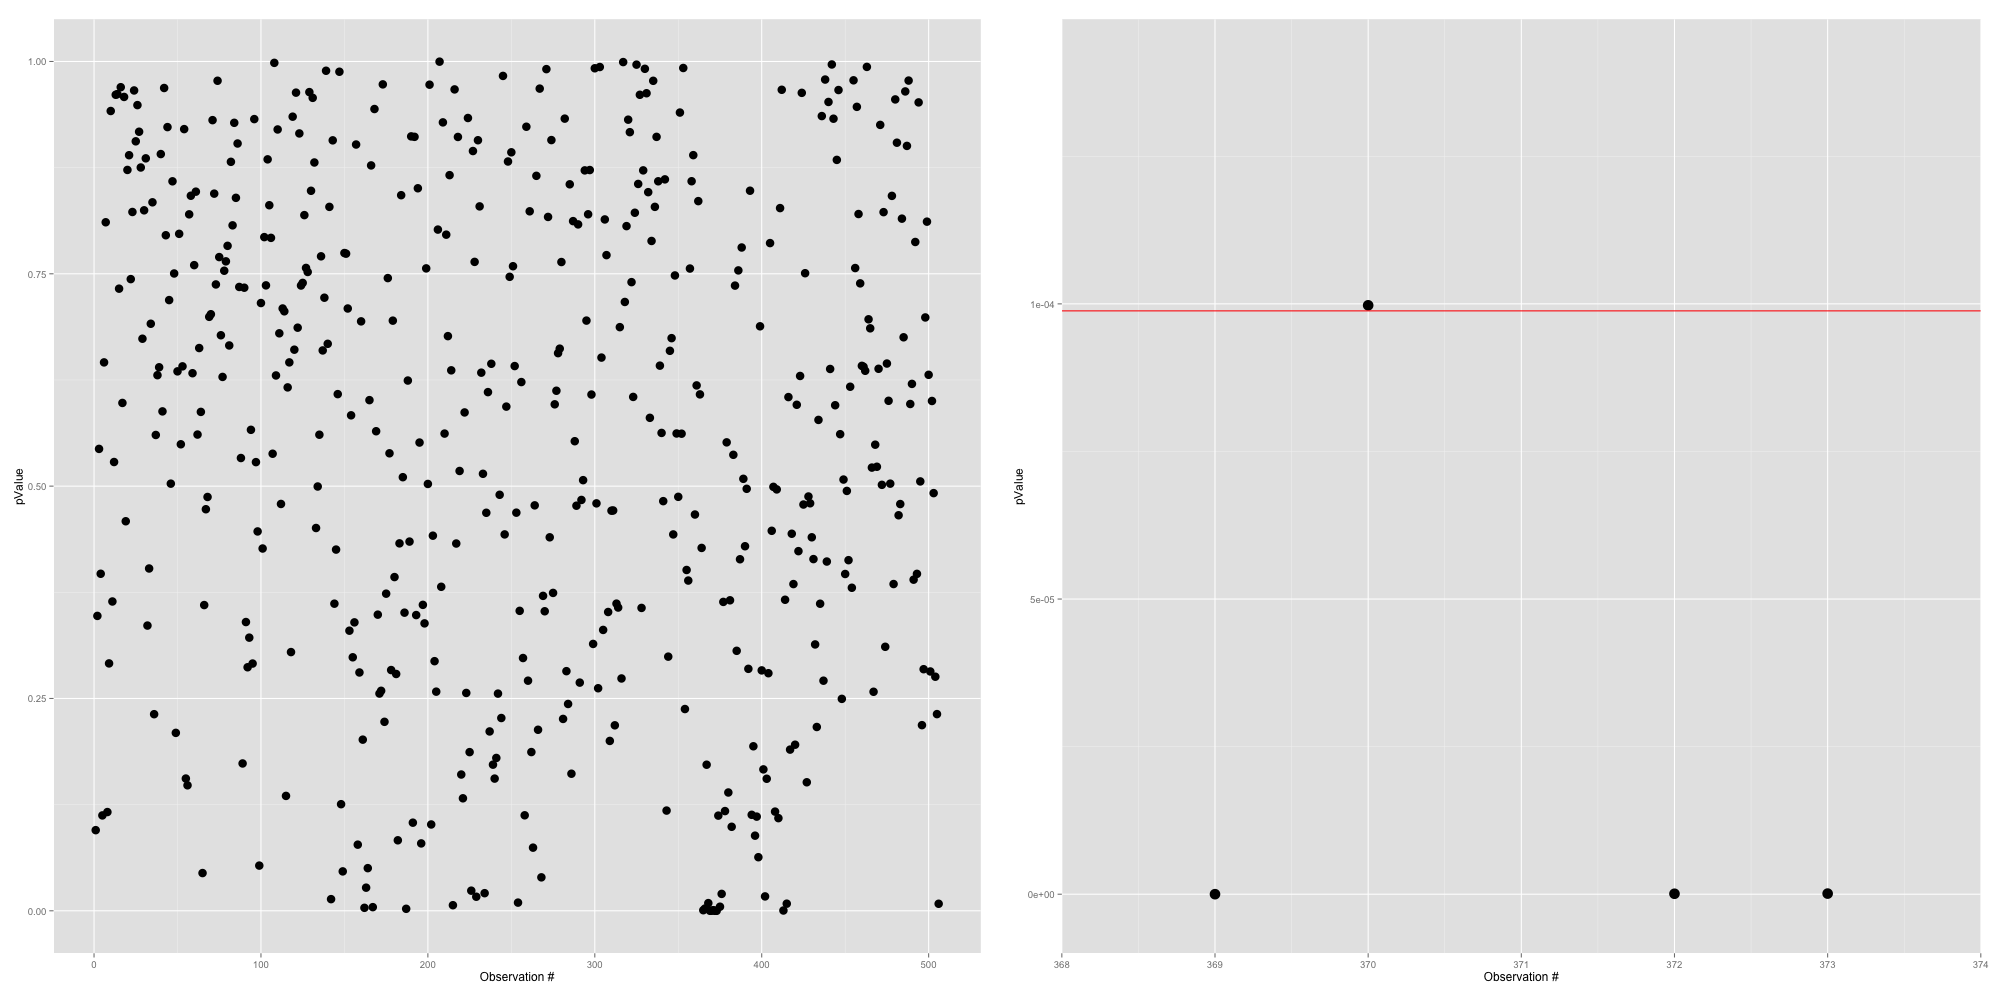
\includegraphics[width=100mm]{pValues.png}
\caption{All p-values are on the left.  Influential observations with the Bonferroni-corrected critical value are on the right.}
\end{figure}


\section{Results and Conclusions}
\subsection{The Fit}
\lstinputlisting{./summary.R}

Every variable included in the model is significant, though $chas$ is on the borderline.  I believe this model is one of the best we could use for prediction purposes, up to performing advanced techniques that I am not to familiar with.

\subsection{Interpretation}
Now, we will try to apply the model's results to our questions.  Suppose an area wishes to raise the median value of owner-occupied homes.  It would want to perform better in those categories which would have the greatest impact on this quantity.  The answer to this question lies in the coefficients.  However, the coefficients alone give us no information, since they can only be interpreted with information about the spread of the corresponding explanatory variables.

A valid question to ask is, ``If a tract is currently around the first quartile in some category, what effect would improving to the third quartile have on its median home value?"  Let $Q_i$ and $q_i$ be the third and first quartiles of the $i$th explanatory variable, respectively, and define a statistic $I_i$, called ``improvement" by
$$
I_i = \beta_i(Q_i - q_i)
$$
This statistic accounts for the spread of the data.  One unit of a given quantity is completely arbitrary, but using quartiles gives us a way to compare the categories with each other.  Thus, we might attempt to answer the question of which categories have the highest influence on median home value by ranking them according to the absolute value of this statistic, which is listed in the right column of the below table.

\lstinputlisting{./interpretation.R}

The difficulty with this interpretation is rooted in multicollinearity; many of the explanatory variables exhibit significant relationships with each other.  The best example of this is the variable $dis$, which has a negative coefficient in the full model but a positive coefficient in the simple linear model $MEDV \sim DIS$.  In the full model, $dis$ is being interpreted in the presence of other variables which it has a linear relationship with; it has a positive relationship with $londist$ and $zn$, but a negative relationship with $nox$ and $age$.  We can no longer interpret the effects of increasing $dis$ in this way, since it assumes we hold all other variables constant.  The truth is that any reasonable increase in $dis$ would necessitate a response in these four other variables that we are not taking into account.

It is possible to account for these relationships and interpret this model, though the results would be too complicated to comprehend.  For instance, we might look at the the effect on $medv$ of moving from the third to first quartile in $dis$ while \emph{also} moving the corresponding amount in each category that $dis$ has a relationship with.  This would amount to looking at the quantity
$$
\sum_{x \in \text{vars}} \beta_{x \sim dis} \beta_{dis} (Q_{dis} - q_{dis})
=
I_{dis} \sum_{x \in \text{vars}} \beta_{x \sim dis}
$$
where $\beta_{dis}$ is the coefficient of $dis$ in our model and $\beta_{x \sim dis}$ is the coefficient of $x$ in a simple linear regression of $x$ against $dis$.  This expression returns a positive value, while earlier the percieved impact of $dis$ was negative.  So even the signs of the coefficients in this model cannot be trusted.  Of course, this formula does not account for other relationships between explanatory variables, and so is also not valid.  To take them all into account simultaneously would be mathematically complicated, but even more problematic is that the resulting value would be impossible to decide which variable should be viewed as the independent cause of the increase.

This model is built for prediction.  It is too large and inclusive to be used effectively for interpretation.  If we are interested in understanding the relationship between each variable and the target variable, we would want to build a smaller model.  Otherwise, we are forced to interpret the variables in the presence of each other, which becomes increasingly complicated as the model grows and multicollinearity arises.

Furthermore, this model includes variables that could not even be interpreted in a simple linear regression.  For instance, what is $b$?  A measure of the population's deviation from $63 \%$ black?  Does this have any meaning at all?  Possibly all it does is add a degree of freedom to help the model fit a plane to the data, while in truth it has no reasonable relation to $medv$ whatsoever.

I have used an alternative variable selection method to produce a smaller model.  First, I eliminated variables that are not useful in explaining $medv$.  Specifically, these were $b$ and $lstat$.  Clearly, having many lower status people in the population correlates with low property values, however a lower status population is likely caused by the fact that those people can afford to live there, i.e. the median home value is low.

Next, I worked backwards from the full model, eliminating variables that did not satisfy a criteria that measures a variable's desirability based on its significance in the model and its correlation with the other explanatory variables present.  After doing this several times, using various cutoff values, the model eventually produced was
$$
MEDV = RM + PTRATIO + CRIM
$$
A summary is given below.
\lstinputlisting{./summary2.R}
\lstinputlisting{./interpretation2.R}

Using this smaller model, interpretation becomes realistic.  Notice that the signs of the coefficients actually align with how our intuition says those variables should affect property value.  This is because the variables present are relatively uncorrelated (cor$(crim,rm) = -0.2176540$, cor$(crim,ptratio) = 0.2867482$, cor$(rm,ptratio) = -0.3552455$).  Therefore, we can actually talk about the effects of improvement in one of these categories on median home value, without getting lost in the corresponding effects on the other categories.  

It appears that the most important factor is the number of rooms per dwelling, followed by the ratio of pupils to teachers.  Crime rate is relatively less important.  Having big houses with many rooms is probably something that only the home-owners themselves can control, but at least we could tell city council to spend its money on more teachers, not on a bigger police force.

\begin{comment}
From the first two categories, it appears that the ability to get to work is highly influential in determining home values.  The percentage of lower status of the population cannot truly be seen as a cause of low home values; rather, it is probably the other way around.  High tax rates appear to be the next factor in keeping property values low.  Again, having few rooms per dwelling may be something that would only be improved by bringing more wealthy inhabitants into the tract.  It is likely not a cause of, but something that varies with home value.  Nitric oxide emissions may be a misleading category.  While these emissions are produced by transportation, they are most heavily produced by agriculture.  So low home values in areas with high nitric oxide emissions may actually be caused by the fact that they are more rural areas.  This is just speculation, and would require more investigation to determine.  Pupil-teacher ration is the final category, and it's no surprise that good schools bring up home values.
\end{comment}

\section{Appendix}
\subsection{Plots}

\begin{figure}[hp]
\centering
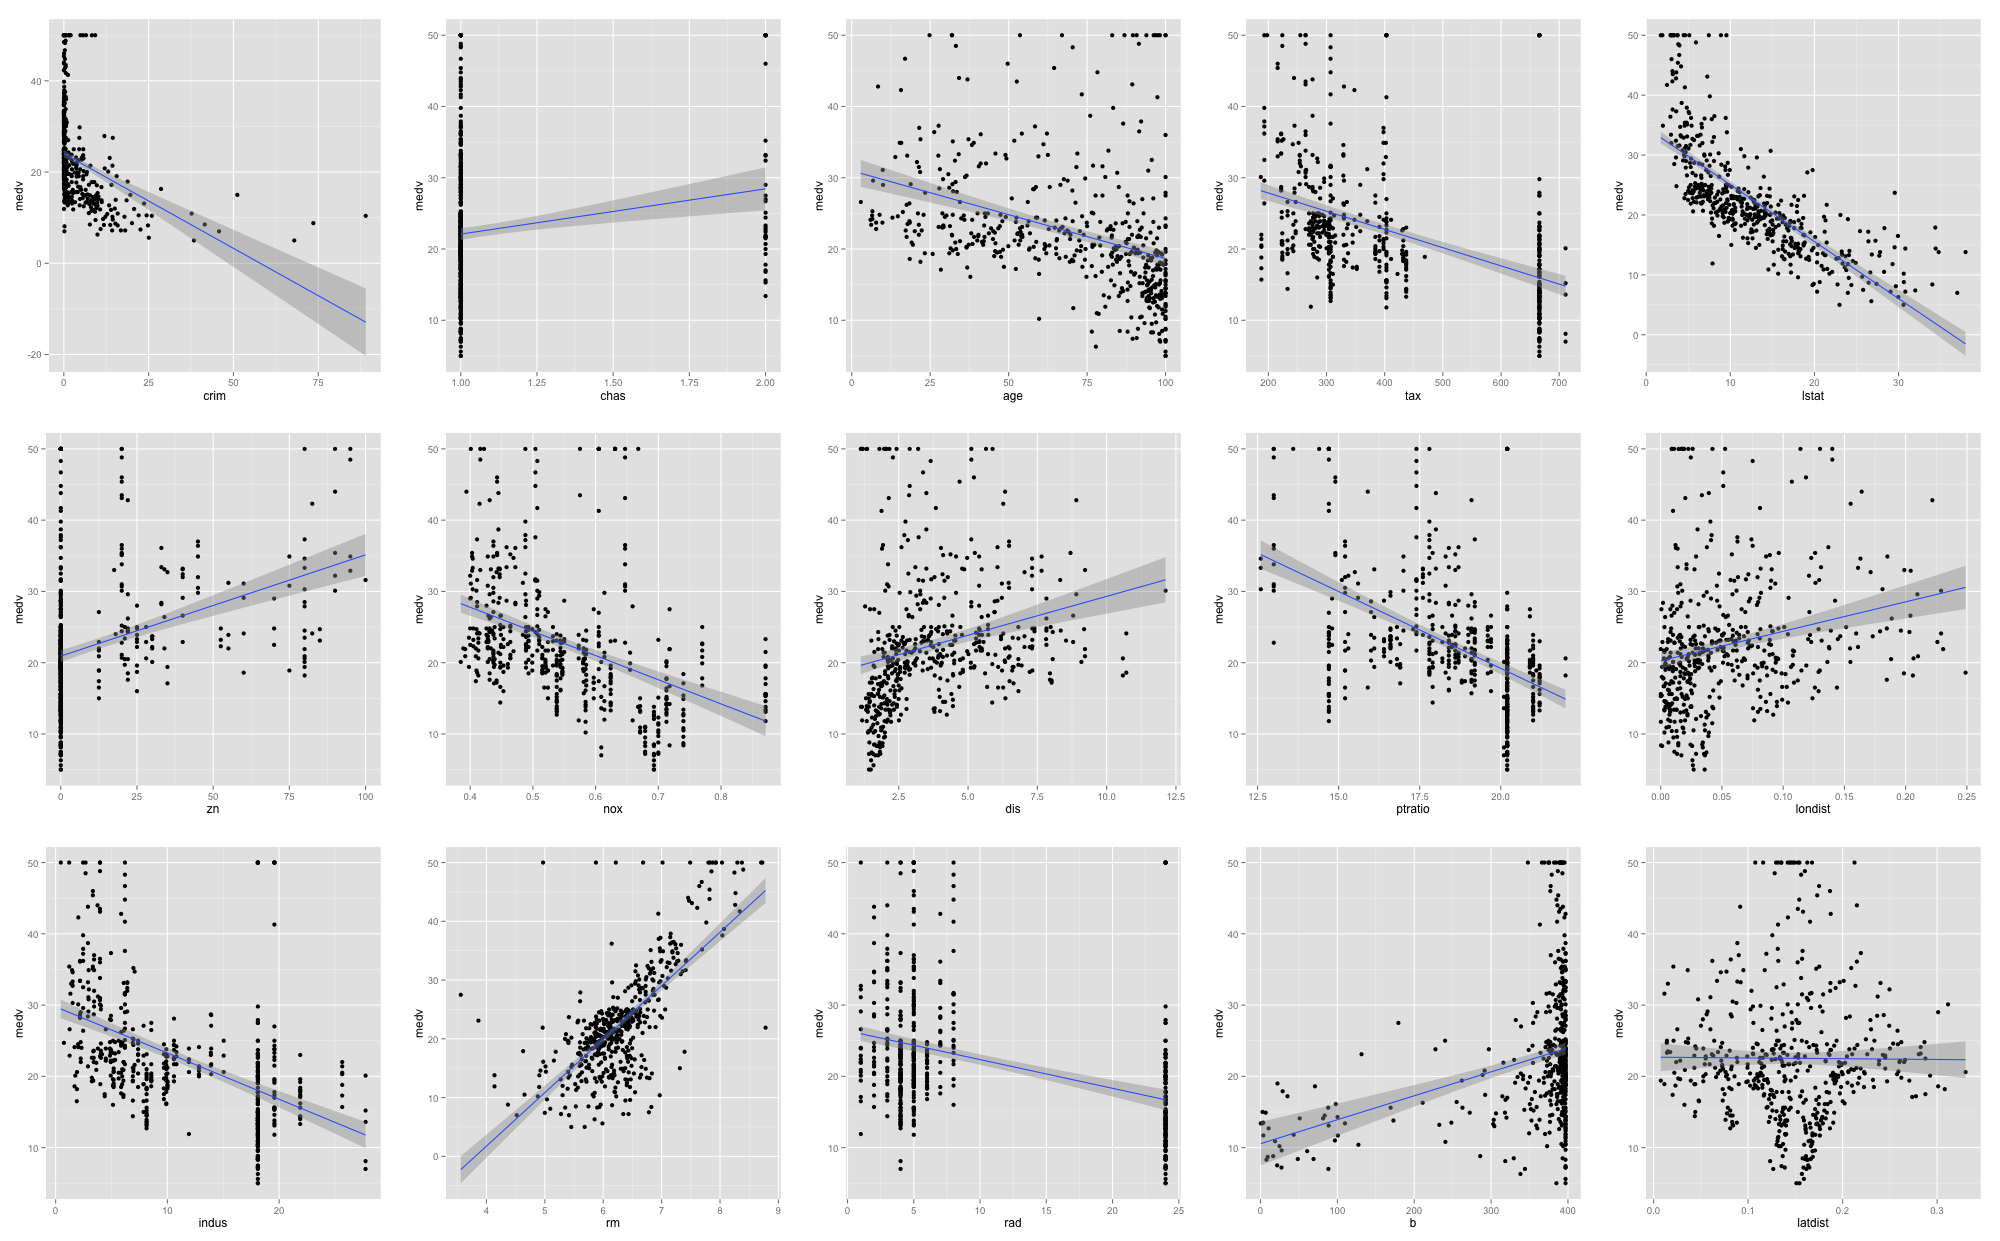
\includegraphics[width=180mm]{simpleplots.png}
\caption{Median value of owner occupied homes plotted against and fit to each individual explanatory variable.}
\end{figure}

\begin{figure}[hp]
\centering
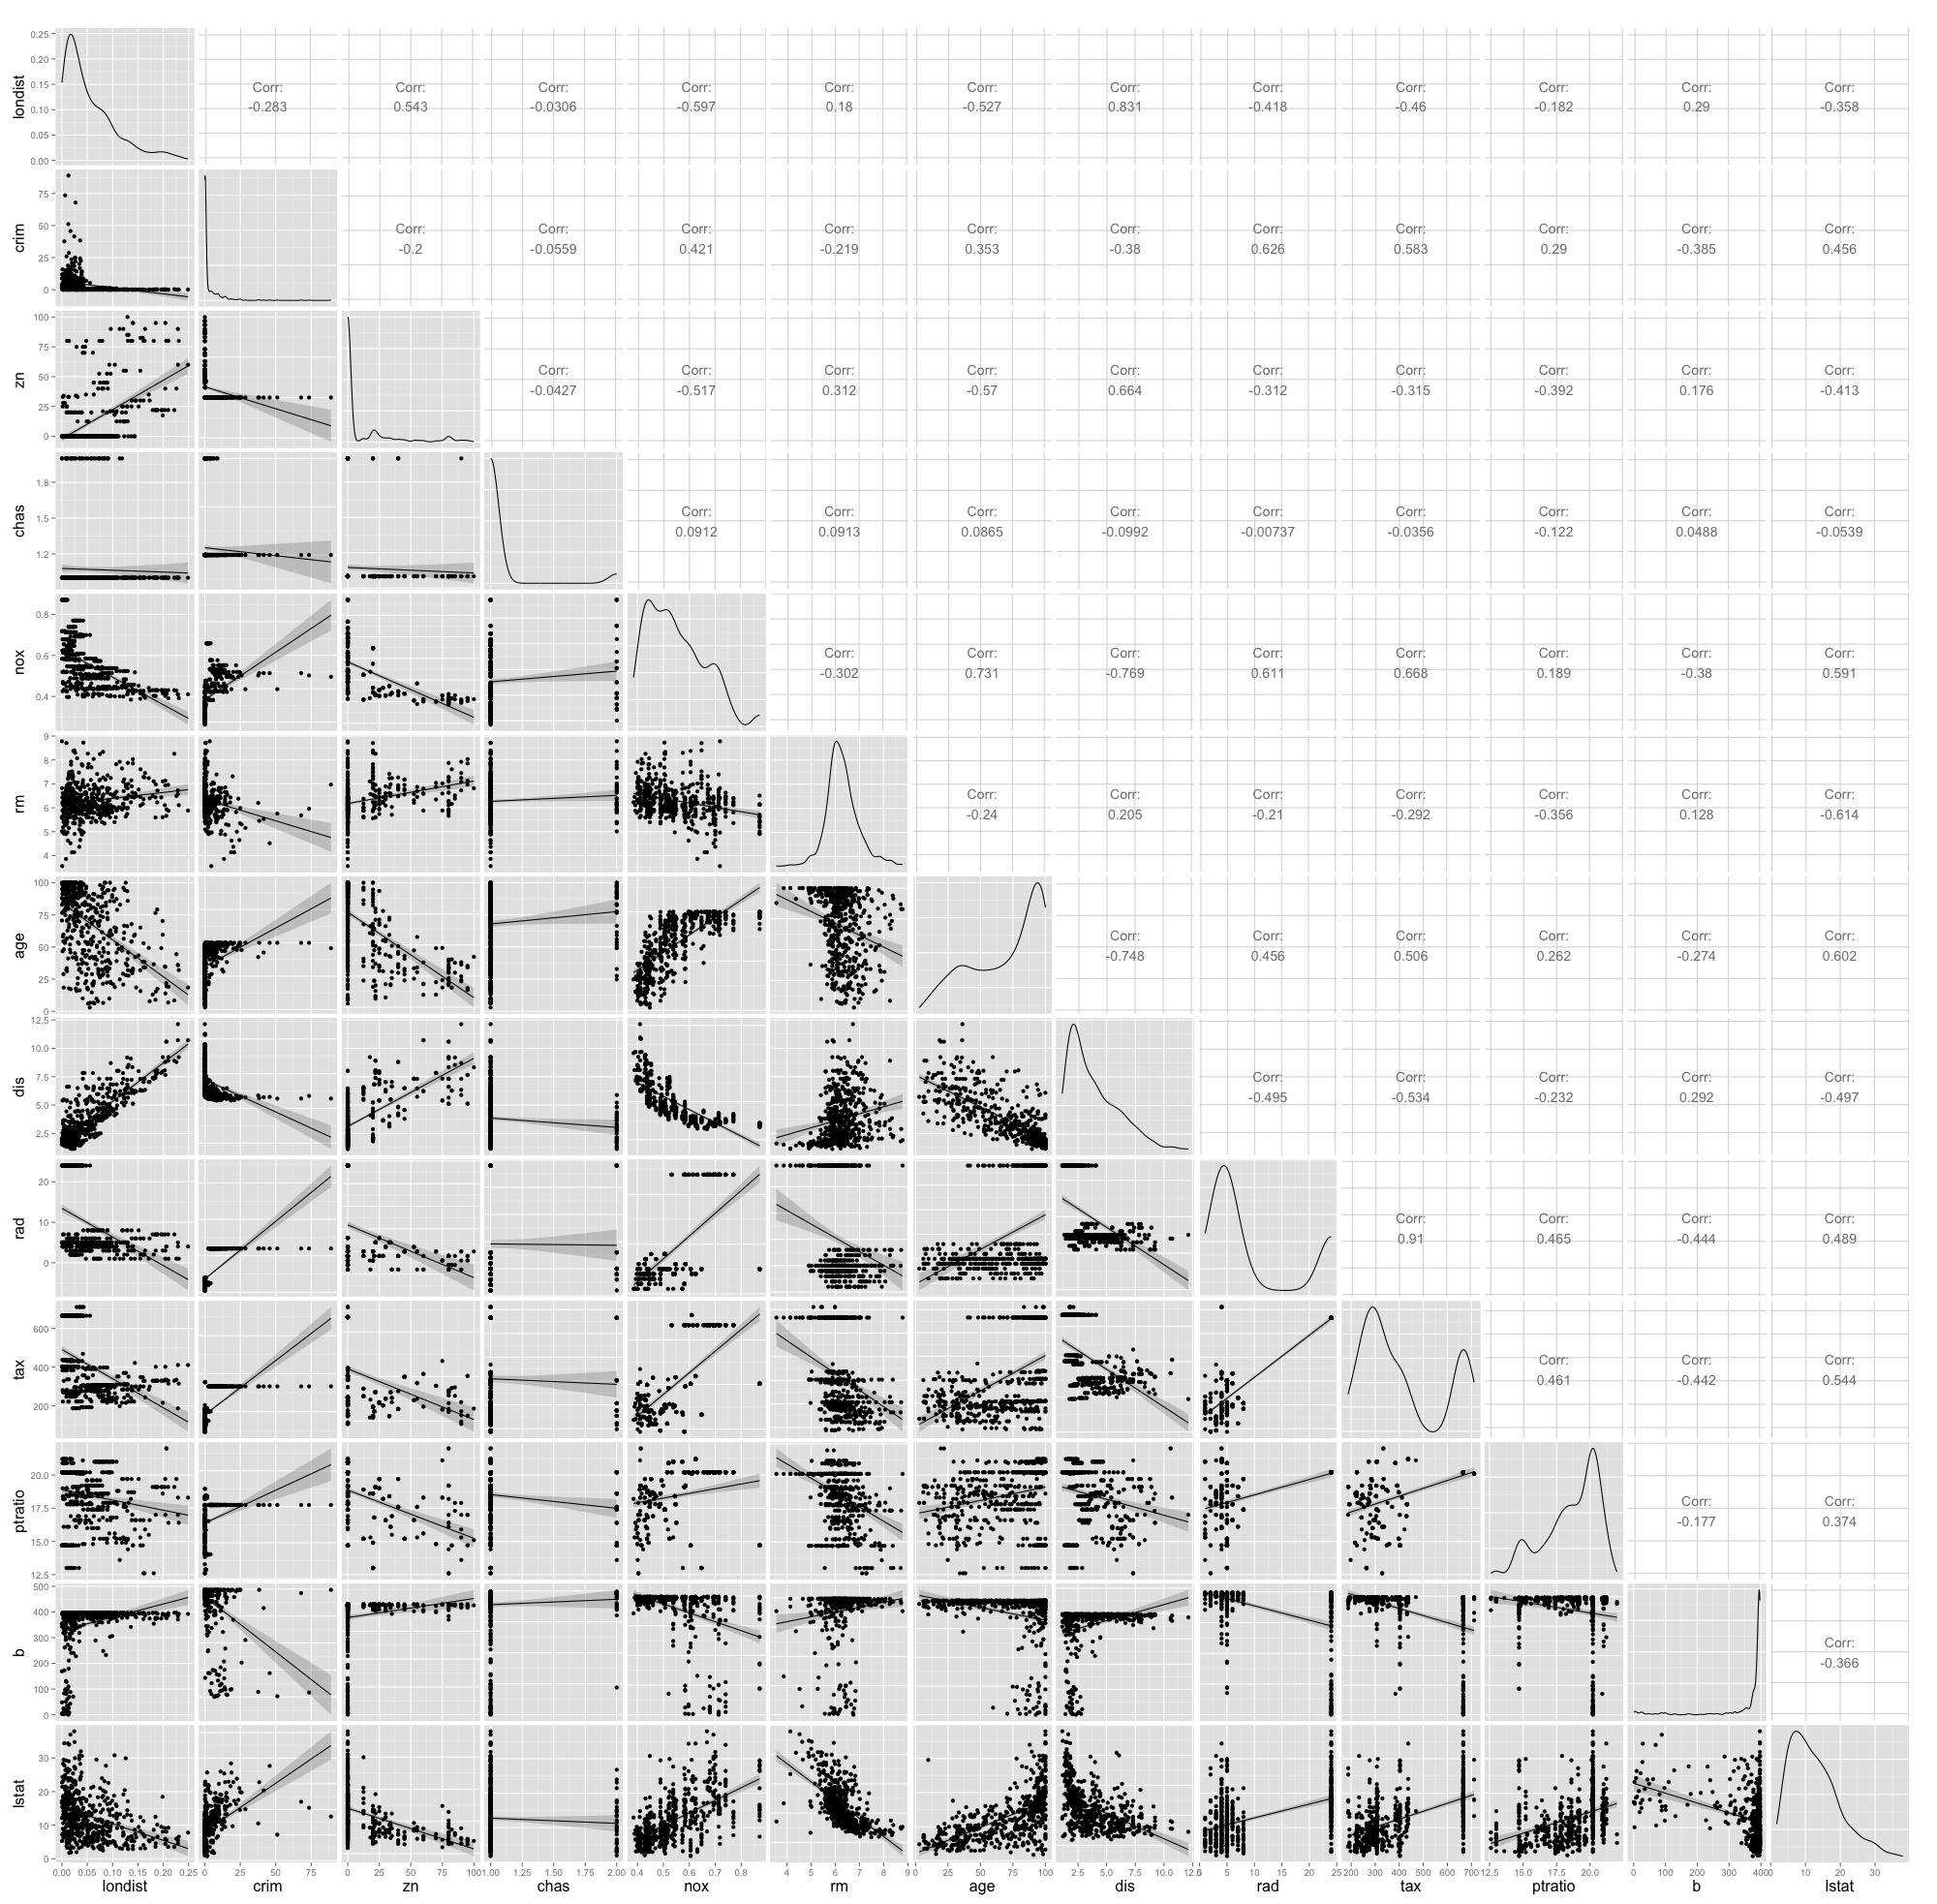
\includegraphics[width=180mm]{pairs.png}
\caption{Pairwise plots of explanatory variables against one another (only those used in the final model) along with lines of best fit are below the diagonal.  Distribution of explanatory variabales are on diagonal.  Correlations are above diagonal.}
\end{figure}

\begin{figure}[hp]
\centering
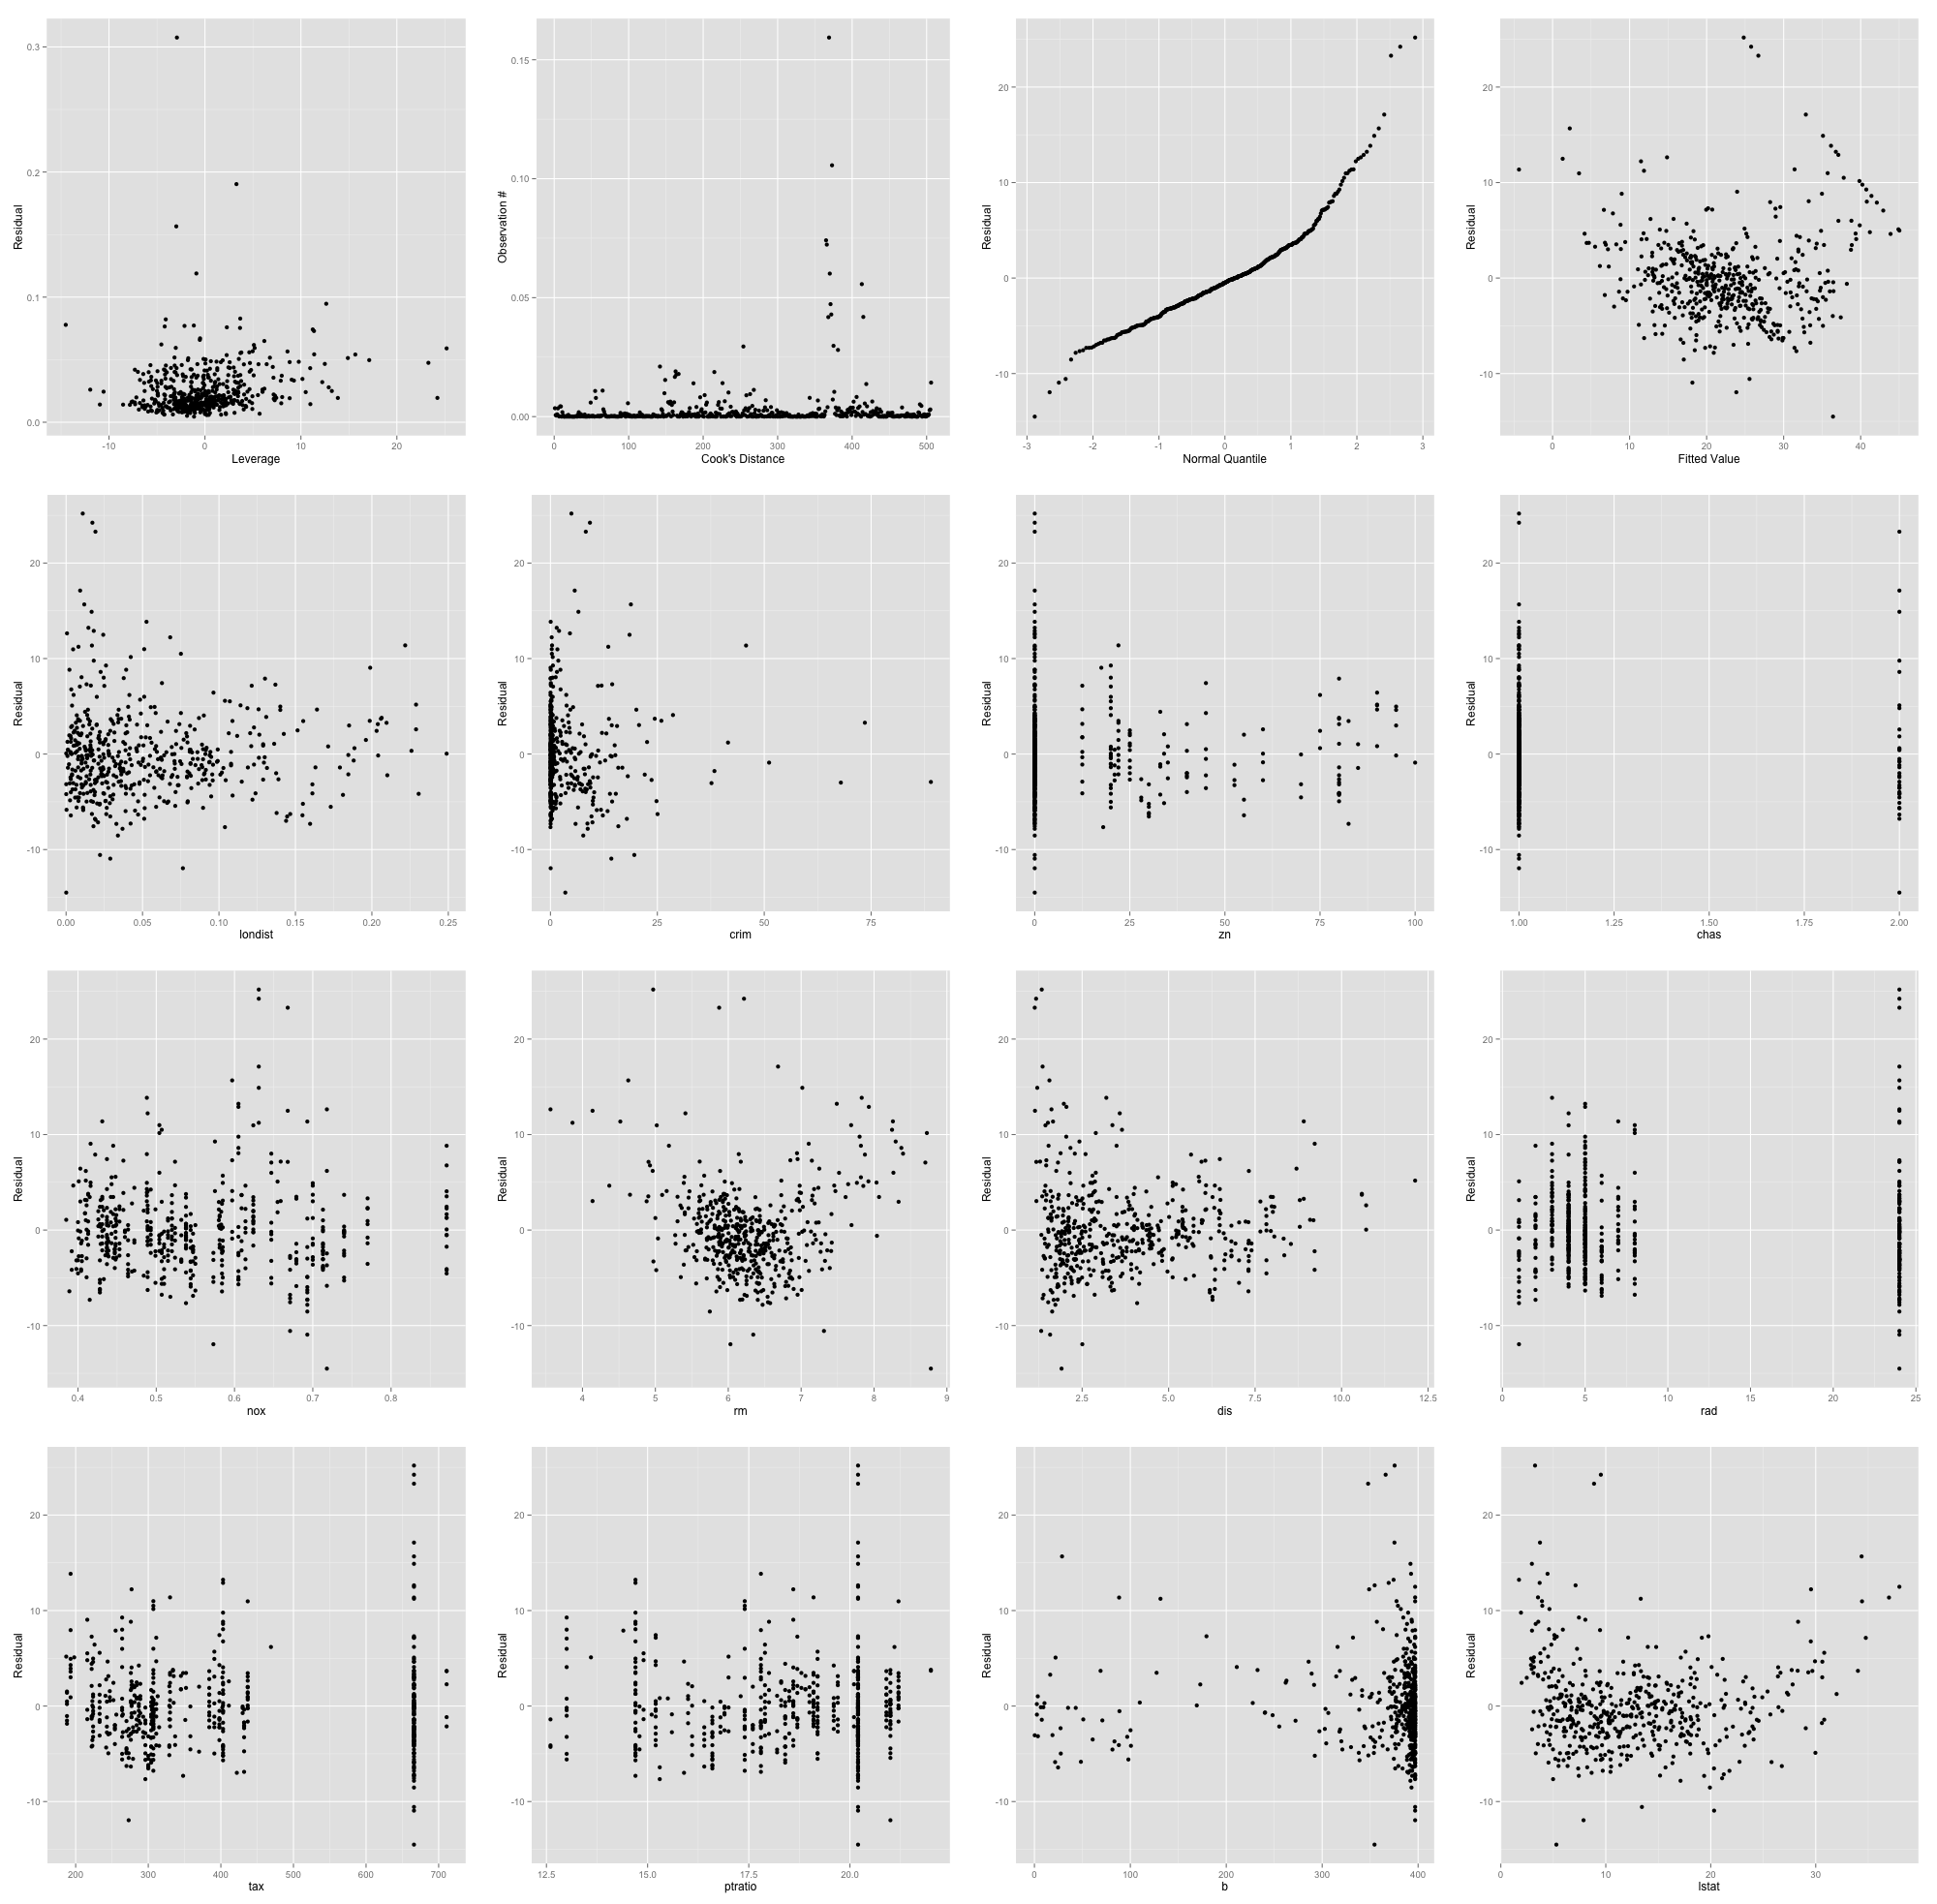
\includegraphics[width=180mm]{diagnostics.png}
\caption{Diagnostic plots for testing the assumptions of the linear model.}
\end{figure}

\pagebreak

\subsection{Code}
\subsubsection{Data Analysis}
\lstinputlisting{./data.R}
\subsubsection{Variable Selection}
\lstinputlisting{./modelselection.R}
\subsubsection{Regression Diagnostics and Outlier Elimination}
\lstinputlisting{./outliers.R}
\subsubsection{Interpretation}
\lstinputlisting{./interpretationcode.R}
\end{document}

















